Cuda is a parallel programming framework from Nvidia that allows programmers to make use of GPU hardware for general purpose computation through the use of language extensions and an API. Prior to the release of Cuda, using GPUs for general computations required advanced graphics programming knowledge. 
\subsection{How Cuda Works}
High performance GPUs (graphics processing units) have become common in commodity hardware. Performing high speed graphics calculations benefits from a massively parallel collection of simple, specialized processors, as graphics related operations tend to follow a SIMD (single instruction multiple data) execution model. GPUs have therefore evolved to provide just this characteristic: a massively parallel multi-core system highly tuned to perform similar calculations on many cores.

A typical cuda program might implement the following steps:
\begin{itemize}
    \item Load data from CPU memory to GPU
    \item Launch specially written kernel functions on the GPU from the CPU
    \item GPU executes computation in parallel
    \item Retrieve data from GPU memory to CPU
\end{itemize}

It is rather simple to begin writing parallel cuda code for execution on a GPU. Challenges arise, however, when trying to optimize codes for proper use of the GPU memory hierarchy, thread grouping and allocation, and tuning for specific hardware. 

\subsection{Cuda Implementation: Iterative}
The iterative form of the FFT algorithm is well suited for execution on a GPU. The strategy will be to treat each executing thread as single entry in the array. That is, each thread is responsible for computing the FFT value of the array location given by its global index. 

Three kernels are used to perform this task: \texttt{bit\_reverse\_kernel()}, \texttt{fft\_kernel\_shared}, and \texttt{fft\_kernel\_finish()}. The sequence of execution in the FFT computation goes like this:
\begin{itemize}
    \item Load input data from CPU to GPU
    \item call \texttt{bit\_reverse\_kernel()} to perform array index bit-reversal in global memory
    \item call \texttt{fft\_kernel\_shared} to perform the partial FFT using shared memory
    \item loop over \texttt{fft\_kernel\_finish()} to finish the FFT in global memory
    \item Retrieve data from GPU memory to CPU
\end{itemize}

This implementation computes all the partial FFTs in shared memory. That is, due to the thread block-size restriction of 1024 threads, this approach was not able to continue with shared memory after the FFT 1024-point FFT has been performed. The limitations were that thread synchronization during kernel execution is limited to the threads within a block, and that threads from neighboring blocks cannot access each other's shared memory.

After the shared memory computation has finished, the CPU code loops over the \texttt{fft\_kernel\_finish()} kernel, which performs one iteration of the iterative FFT loop. This was thought to be necessary so that global device synchronization could be achieved. Otherwise, since the FFT algorithm now needs to reach beyond the limits of thread-block size to continue ($m/2 > 512$), there is the potential to introduce race a condition as each block proceeds out of sync with the others. 

We implemented only the iterative FFT in cuda due to the natural programming style of GPU computations: GPUs are not ideally suited for recursive tasks. However, it is now possible to launch new grids of threads from an executing grid, where previously new grids (kernels) could only be launched from the CPU. This technique is know as Dynamic Parallelism, and enables recursive programming on the GPU. We did not explore this option, but felt it is important to mention.

\subsection{Cuda Analysis}
The performance of our cuda FFT is shown in figure \ref{cudaRuntimes}. This graph includes the numpy FFT, our cuda impementation, and the Nvidia CUFFT library function. For both cuda algorithms, full times and ``inner" times are plotted. The full time includes data transfer from CPU to GPU and back, and the inner time measures only the actual FFT computation.

Several interesting features are visible on the graph. Most obvious is that for both cuda implementations, the total time is dominated by the data transfer. Since this time is nearly constant, and the amount of data being transferred is fairly small, it is reasonable to assume that this is due to communication latency across the PCI-E bus. For $N<1024$, the sequential numpy FFT outperforms either cuda implementation. Between 1024 and $2^{15}$, both cuda implementations grow very slowly. After $2^{15}$, however, the cuda codes start to grow with the same slope as the numpy FFT. This makes sense: the GPUs available on Stampede are Nvidia K20m cards, which have can run a maximum of 26624 concurrent threads. The number $26624 \approx 2^{14.7}$, so the turning point in the cuda performance curve at about $2^{15}$ is expected. Even for large values of $N$, however, our implementation performs about 10 times faster than numpy, and the built-in CUFFT is about 100x faster.

\begin{figure}
    \centering
    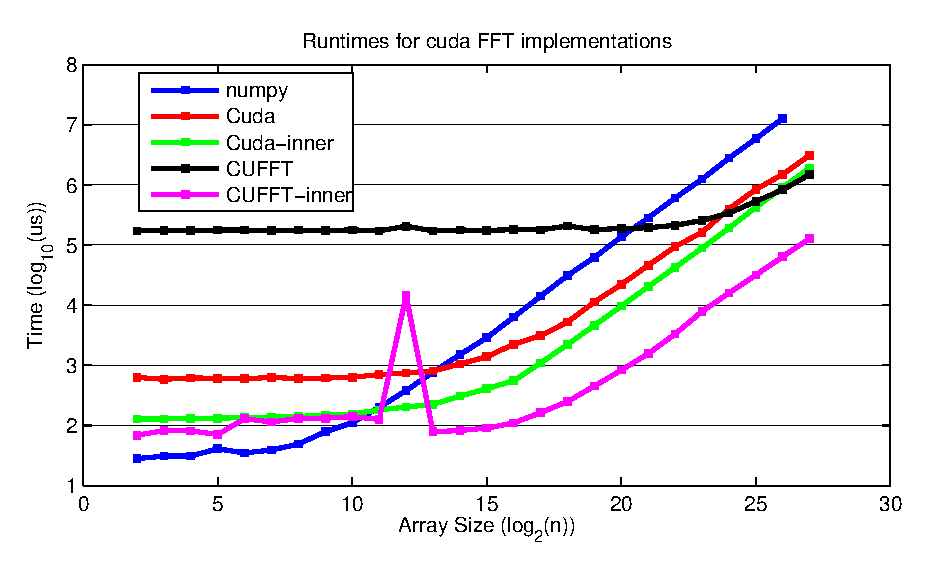
\includegraphics{img/cudaRuntimes.eps}
    \caption{Comparison of cuda FFT runtimes.}
    \label{cudaRuntimes}
\end{figure}